\section{Deep Reinforcement Learning}
In contrast to the manually developed algorithm, a Deep Q-learning based search algorithm was also developed. The agents is trained in using the simple simulator to search the map. Reinforcement learning suits this problem well as can coverage serve a {\color{red} good} reward function. Traditional Q-learning methods store a table of discrete state-action pairs and their expected reward in memory {\color{red}[SOURCE]}. This table is called a Q-table. However, in real world applications state is often continuous, which creates the need to {\color{red} disoretize} the agent state. Another problem is that the size of the Q-table grows with the state space. Neural networks solve both of these problems. The Q-table can be approximated by using a neural network and then used to pick an action given a state.

\subsection{Network}

\subsection{Reward}

\subsection{Training}

\subsubsection{Generating Training Environments}
As to not overfit the network, it must be trained on many different environments. A simple program was created to generate worlds populated by line and circle obstacles.

\def\w{0.31\textwidth}
\begin{figure}[H]
    \begin{subfigure}{\w}
        \makebox(\textwidth, \textwidth)[\textwidth]{
            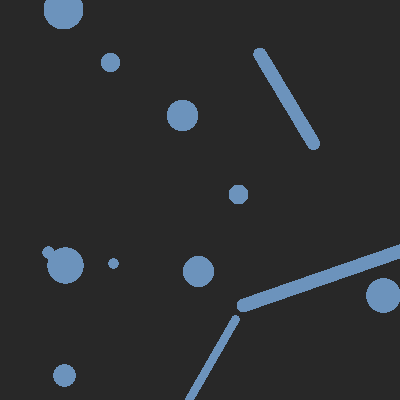
\includegraphics[width=\linewidth]{figures/generated-worlds/world_0.png}
        }
    \end{subfigure}
    \hspace*{\fill}
    \begin{subfigure}{\w}
        \makebox(\textwidth, \textwidth)[\textwidth]{
            
\includegraphics[width=\linewidth]{figures/generated-worlds/world_1.png}
        }
    \end{subfigure}
    \hspace*{\fill}
    \begin{subfigure}{\w}
        \makebox(\textwidth, \textwidth)[\textwidth]{
            
\includegraphics[width=\linewidth]{figures/generated-worlds/world_2.png}
        }
    \end{subfigure}

    \vspace{4mm}

    \begin{subfigure}{\w}
        \makebox(\textwidth, \textwidth)[\textwidth]{
            
\includegraphics[width=\linewidth]{figures/generated-worlds/world_3.png}
        }
    \end{subfigure}
    \hspace*{\fill}
    \begin{subfigure}{\w}
        \makebox(\textwidth, \textwidth)[\textwidth]{
            
\includegraphics[width=\linewidth]{figures/generated-worlds/world_4.png}
        }
    \end{subfigure}
    \hspace*{\fill}
    \begin{subfigure}{\w}
        \makebox(\textwidth, \textwidth)[\textwidth]{
            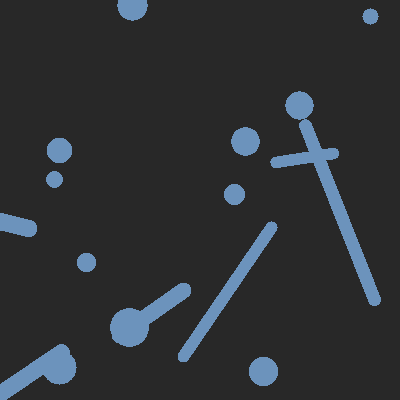
\includegraphics[width=\linewidth]{figures/generated-worlds/world_5.png}
        }
    \end{subfigure}
    \caption{Examples of generated environments} \label{fig:generated-enviornments}
\end{figure}

\end{document}
